\chapter{Research gap analysis}
\label{chap:research-gaps}

The literature synthesis conducted in \cref{chap:literature-review} reveals a fundamental disconnect between theoretical radar polarimetry and its practical implementation in automotive millimetre-wave sensors.
While polarimetric decomposition methods are well established in stationary remote sensing and \gls{sar}, their direct application to dynamic road environments is hampered by grazing incidence geometry, severe clutter coupling, micro-Doppler dynamics, and strict multiplexing constraints.
Concurrently, modern \gls{mimo} radar topologies and front-end antenna structures are overwhelmingly optimized for scalar angular resolution, treating polarization as an unmanaged or secondary parameter.
This results in array manifolds plagued by cross-polar leakage, phase-centre displacement, and polarization squint across the virtual aperture.

To resolve these combined challenges, this chapter establishes the academic and methodological framework of the doctoral project.
First, \cref{sec:hypotheses} translates the identified limitations into a structured hierarchy of primary and secondary research questions, detailing the domain transfer hurdles from remote sensing to automotive radar.
\Cref{sec:gaps-identified} categorizes the precise technical gaps spanning polarimetric target models, front-end antenna hardware, and \gls{mimo} array synthesis.
\Cref{sec:proposed-solutions} outlines the proposed technical methodology, including perturbation analysis for algorithm-driven antenna requirements, a polarimetric scattering simulator, and \enquote{polarimetry-first} virtual array topologies.
Finally, \cref{sec:feasibility-study} presents a feasibility study and initial design development of an aperture-coupled series-fed array, evaluating high-coupling element matching, progressive phase compensation, and corporate feed transitions at X-band as a baseline for W-band scaling.


\section{Formulation of hypotheses and research questions}
\label{sec:hypotheses}

Addressing the key bottlenecks of automotive polarimetry requires formulating precise, testable hypotheses that link physical scattering physics to array manifold design.
This section outlines the overarching primary research question alongside three supporting sub-questions, and articulates the physical domain transfer challenges encountered when adapting remote sensing polarimetry to dynamic, near-field automotive scenarios.

\todo{Update research questions.}
\begin{custombox}{Research questions}
    \begin{itemize}
        \item \textbf{Primary research question:} Can the integration of a high-resolution $12 \times 16$ \gls{mimo} architecture with Doppler-resolved polarimetric processing significantly enhance the classification accuracy of dynamic \glspl{vru}?
        \item \textbf{Secondary research question 1:} What is the optimal choice of polarization basis for polarimetric automotive radar?
        \item \textbf{Secondary research question 2:} What are the fundamental lower bounds on antenna requirements (e.g. cross-polarization discrimination, phase centre alignment), as derived from the sensitivity and robustness of polarimetric decomposition algorithms?
        \item \textbf{Secondary research question 3:} How can \gls{mimo} topologies be optimized specifically for polarimetric fidelity -- establishing \enquote{polarimetry-first} array designs -- to mitigate the detrimental effects of phase centre displacement and cross-polar coupling?
    \end{itemize}
\end{custombox}

\subsection{Domain transfer challenges}

The polarimetric decomposition techniques reviewed in \cref{sec:incoherent-decomposition} were historically developed for \gls{sar} and spaceborne remote sensing, operating under implicit assumptions of static scenes, far-field plane-wave incidence, and steep incidence angles.
Transferring these mathematical formulations to W-band automotive radar introduces several physical and operational challenges:

\begin{enumerate}
    \item \textbf{Grazing incidence and surface suppression.} Automotive radars operate near the ground plane (\qtyrange{0.3}{1.5}{m} mounting height), resulting in grazing incidence angles (\qtyrange[range-units=repeat]{85}{89}{\degree}). At these angles, pseudo-Brewster angle and rough surface scattering mechanisms dictate that vertical polarization backscatter from asphalt and concrete exceeds horizontal returns. This surface anisotropy, which was demonstrated by \textcite{visentinPolarimetricRadarAutomotive2019,bouwmeesterRoadSurfaceConditions2023}, artificially inflates differential reflectivity $Z_{\mathrm{DR}}$ and biases target decomposition parameters such as the Pauli $\alpha$ angle, distorting the inferred physical scattering mechanism.
    \item \textbf{Nonstationary across coherent integration intervals.} In satellite or airborne \gls{sar}, the observation duration over a homogeneous land-cover parcel is sufficiently long to accumulate independent samples for forming a well-conditioned coherency matrix $\vec T$ (or covariance matrix $\vec J$). In dynamic automotive driving scenarios, targets such as pedestrians or cyclists move across spatial resolution cells on millisecond timescales. Estimating the coherency matrix via spatial or temporal windowing assumes local stationarity -- a condition frequently violated by fast-moving \glspl{vru} and rapidly evolving clutter.
    \item \textbf{Micro-Doppler and polarimetric coupling.} Standard polarimetric target decompositions treat the target as a single static or rigid body, disregarding velocity distribution. However, for articulate \glspl{vru}, the polarimetric signature is inherently time-variant and coupled with the micro-Doppler spectrum. For example, a pedestrian's torso exhibits a stable co-polarized single-bounce response, whereas swinging limbs generate transient cross-polarized depolarization at distinct Doppler offsets.
\end{enumerate}

These discrepancies indicate that while classical remote sensing decompositions provide a foundational framework, they cannot be directly ingested by automotive classification pipelines without explicitly accounting for grazing geometry, nonstationary, and micro-Doppler coupling.

\subsection{Doppler-resolved polarimetry and automotive operational hurdles}

Expanding polarimetric analysis into the joint Doppler-polarization domain offers a promising path forward, but it must contend with severe hardware and environmental constraints unique to vehicle integration:

\begin{itemize}
    \item \textbf{Near-field wavefront curvature.} Operating ranges in urban driving (\qtyrange{5}{60}{m}) fall within the transition region between the near-field and far-field for large \gls{mimo} virtual apertures. Plane-wave incidence assumptions break down, introducing range-dependent phase errors across the array manifold that corrupt cross-polar phase calibration if left uncompensated.
    \item \textbf{Multipath dominance and depolarization.} Ground reflections, metallic vehicle bodies, and roadside structures create multi-path propagation channels. Double-bounce reflections off the road surface and vehicle undercarriages introduce spurious cross-polar energy, generating depolarization characteristics not accounted for by free-space target models.
    \item \textbf{Multiplexing constraints and Doppler ambiguity.} Achieving dual-polarized operation in a \gls{mimo} system requires switching polarizations either across transmit pulses or receive channels. In \gls{tdm}-\gls{mimo}, sequential polarization switching extends the \gls{pri} per virtual channel, compounding phase wrapping and velocity ambiguity in high-speed traffic.
\end{itemize}

These operational hurdles justify the development of joint spatial-Doppler-polarimetric processing schemes and \enquote{polarimetry-first} array manifolds designed specifically to preserve phase coherence and polarimetric fidelity under tight automotive form factors.


\section{Research gaps identified in literature}
\label{sec:gaps-identified}

Although individual aspects of millimetre-wave radar, \gls{mimo} virtual aperture synthesis, and polarimetric decomposition have been studied independently, their intersection remains largely unmapped.
This section summarizes the three critical gaps identified in current literature: the lack of Doppler-resolved spatial scattering models, the absence of algorithm-driven front-end requirements, and the omission of polarization purity in \gls{mimo} topology synthesis.


\subsection{Gaps in polarimetric models}

The decomposition methods discussed in~\cref{subsec:coherent-decomposition,sec:incoherent-decomposition} generally treat the radar target as a singular spatial entity.
However, for dynamic \gls{vru} classification, a purely spatial perspective is insufficient.
Pedestrians and cyclists are articulate structures characterized by complex motion, generating a unique spectral signature known as the \emph{micro-Doppler} effect.

While micro-Doppler analysis is conventionally performed on scalar spectrograms, the physical scattering mechanisms of limbs and wheels are non-stationary.
Therefore, the polarimetric features should theoretically vary as a distributed function over the Doppler domain.

\paragraph{Validation of the polarimetric-Doppler hypothesis.}
Recent experimental work has validated the conjecture that resolving polarimetry in the Doppler domain yields distinct, semantic classification features.
As demonstrated by \textcite{bouwmeesterClassificationDynamicVulnerable2025}, the scattering mechanisms of \glspl{vru} are not constant but evolve across the gait cycle.
Using a standard $3 \times 4$ \gls{mimo} configuration (producing $12$ virtual channels) in a diagonal polarization basis, the study confirmed that specific micro-Doppler components exhibit unique polarimetric behaviours:
\begin{itemize}
    \item \emph{Cyclists:} While the frame and rider exhibit dominant odd-bounce scattering (high Pauli $a$ and $b$ features), the rear wheel introduces a distinct cross-polarized response (Pauli $c$ feature) corresponding to a dihedral mechanism, likely due to the spoke-rim interaction.
    \item \emph{Pedestrians:} The torso and forward-swinging limbs exhibit predominantly co-polarized returns, whereas backward-swinging limbs show weak depolarization.
\end{itemize}
By feeding these Doppler-resolved polarimetric power maps into a convolutional neural network, an F1-score of $98.2\%$ was achieved, statistically outperforming single-polarization baselines and confirming the utility of the feature set.

\paragraph{Environmental clutter semantics and road features.}
Beyond \gls{vru} limb motion, polarimetric signatures offer unique physical mechanisms for environmental scene understanding and road infrastructure classification.
For instance, specular road surface reflections can differentiate dry pavement from water or black ice through co-polar ratio anomalies ($Z_{\mathrm{DR}}$).
Similarly, optical retroreflectors (cataphotes) on guide posts and milestones might exhibit distinct trihedral (odd-bounce) returns at short millimetre waves, whereas road signs present single-plane reflections in contrast to the volume scattering of roadside foliage and the multi-path depolarization of metal lampposts.

\paragraph{The spatial resolution bottleneck.}
Despite validating the phenomenological benefits of polarimetric micro-Doppler, the current state of the art faces a critical limitation regarding spatial separability.
To manage the computational load and the limited angular resolution of a standard $12$-channel virtual array, the processing pipeline proposed by~\textcite{bouwmeesterClassificationDynamicVulnerable2025} relies on a \enquote{dominant target} selection strategy. By computing the angle that maximizes the sum of the squared absolute values of the scattering matrix, this procedure isolates the strongest scatterer within a range-Doppler cell and removes the angular dimension from the processed measurement data.

While this approach served as an effective stop-gap to demonstrate the value of Doppler-resolved polarimetry given specific hardware constraints, it is insufficient for complex urban environments.
In a realistic traffic scene, a \gls{vru} is frequently spatially adjacent to strong static reflectors (e.g. fences, guardrails, or parked vehicles).
If a pedestrian and a static object co-exist within the same range-Doppler bin, the polarimetric signature of the dominant clutter will mask the subtler polarimetric features of the \gls{vru} limbs.
Consequently, low-resolution estimates of entropy $H$ and anisotropy $A$ (or similar classification features) become contaminated, rendering the classification features ambiguous.
To advance beyond this limitation, the radar architecture must possess sufficient angular resolution to spatially isolate dynamic \glspl{vru} from clutter \emph{before} polarimetric feature extraction.


\subsection{Gaps in front-end technologies}

A critical gap exists in balancing polarimetric dynamic range with mass manufacturing constraints.
While the industrial baseline (microstrip patches) supports mass production and straightforward integration, it naturally bottlenecks polarimetric fidelity, struggling to maintain necessary \gls{xpd} beyond moderate scan angles.
Dense \gls{mimo} lattices with this technology suffer from severe mutual coupling that distorts the polarization matrix.
Conversely, while emerging integrated waveguide solutions (such as \glspl{gw}) offer the necessary electromagnetic purity and isolation, they are still far from being considered viable for widespread adoption.

Crucially, the literature lacks a formalized framework for deriving antenna performance requirements directly from the sensitivity of the target classification algorithms.
Current hardware design often proceeds in isolation from the signal processing pipeline.
Consequently, the fundamental lower bounds on antenna specifications -- such as the maximum allowable phase error or amplitude imbalance before a polarimetric decomposition method fails -- remain undefined.


\subsection{Gaps in MIMO topologies}

The interaction between spatial sparsity, virtual array synthesis, and polarization purity remains largely unexplored in the W-band.
While numerous algorithms exist for scalar 2D array synthesis, extending these to dual polarization reveals profound calibration and performance gaps.
Most published W-band polarimetric prototypes suffer from severe cross-polar coupling, reduced aperture efficiency, and phase centre mismatches.

Specifically, the physical displacement between orthogonal radiating elements (e.g. horizontal and vertical patches) introduces a \enquote{polarization squint} or parallax effect.
Even in co-located \gls{mimo} layouts, the co-polar channels do not share identical phase centres or beam shapes.
As far as the current literature indicates, apart from preliminary investigations into polarimetry with standard \gls{mimo} synthesis~\parencite{zhaoCalibrationPolarimetricAutomotive2024}, there is a distinct absence of \enquote{polarimetry-first} array topologies.
Currently, no established array topology exists that is mathematically optimized from its inception to preserve the fidelity of the full scattering matrix while simultaneously maximizing spatial resolution and multiplexing feasibility.


\section{Proposed solutions and design choices}
\label{sec:proposed-solutions}

To systematically close the identified research gaps, a top-down engineering methodology is proposed.
Rather than relying on trial-and-error hardware iteration, this section presents an algorithm-driven perturbation analysis to derive lower bounds on antenna specifications, a modular simulation framework to model target scattering alongside array phase-centre errors, and novel \enquote{polarimetry-first} virtual array topologies.


\subsection{Derivation of antenna requirements via perturbation analysis}

To bridge the gap between front-end hardware and signal processing, this research proposes a top-down, algorithm-driven methodology for antenna design.
Rather than aiming for absolute electromagnetic perfection, the project will derive the fundamental lower bounds of antenna performance required for robust \gls{vru} classification.

This will be achieved by performing rigorous sensitivity and perturbation analyses on standard polarimetric decomposition methods.
By systematically injecting calibrated noise and systematic measurement errors (modifying polarimetric component amplitudes, phases, and cross-channel phase differences) into ideal scattering matrices, the robustness of the decomposition algorithms will be mapped.
The resulting performance margins will then be translated directly into structural and electrical requirements for the antenna system.


\subsection{Polarimetric scattering and parallax simulator}

To execute the perturbation analysis and study the effects of \gls{mimo} physical displacement, a comprehensive simulation platform will be developed.
This tool will calculate the polarimetric response of a target as measured by a \gls{mimo} array with varied phase centre locations.

The development of this simulator is envisioned as a collaborative effort, partitioning the problem into two domains: the electromagnetic scattering physics of the target and the array embedded radiation patterns extracted using full-wave electromagnetic simulations.
By defining a specific application -- such as classifying vehicles versus pedestrians -- the simulator will compute the scattered field, apply spatial transformations to account for the physical displacement of the polarimetric array elements, and feed the resulting corrupted matrix into the decomposition algorithms.
This will allow for the explicit study of polarization squint and the evaluation of calibration techniques to mitigate systematic measurement errors.


\subsection{Polarimetry-first MIMO topologies}

While the academic literature is rich with novel, optimization-driven antenna concepts, the development of robust polarimetric processing algorithms benefits from a stable hardware baseline.
By utilizing established uniform topologies or industry-standard sparse reference designs, system variability is minimized.
This ensures that observed anomalies in the Doppler-polarimetric domain can be attributed to target scattering physics rather than artefacts of an experimental antenna array manifold.

The integration of polarimetric functionality into \gls{mimo} radar introduces a new dimension to topology synthesis: the management of the dual-polarized signal space.
Unlike scalar \gls{mimo} (one polarization), where the primary goal is maximizing the virtual aperture, polarimetric designs must also ensure the fidelity of the full scattering matrix measurement.
Consequently, the design space splits into two fundamental architectural choices: the use of dual-polarized elements sharing a common phase centre versus the spatial interleaving of single-polarized elements.

Building upon the insights gained from the simulator, this research will pioneer the synthesis of \enquote{polarimetry-first} \gls{mimo} topologies.
By abandoning legacy scalar optimization techniques, the design space will be constrained to topologies that explicitly minimize the phase centre disparity between orthogonal channels.
The project will critically analyse the suboptimal characteristics of existing dual-polarized demonstrators to identify specific topological aspects -- such as sub-array interleaving, virtual channel overlapping, and spatial symmetry -- that can be mathematically optimized to ensure true polarimetric alignment across the synthesized virtual aperture.

\paragraph{Dual-polarized architectures.}
The most theoretically robust approach involves the use of dual-polarized elements at each array position (see \cref{fig:dual_pol_elements}).
In this configuration, orthogonal polarizations (typically horizontal and vertical) ideally%
    \footnote{It is plausible that even with dual-polarized antennas, the phase centres of the co- and cross-polar channels do not perfectly coincide due to manufacturing tolerances, feed network imbalances, or mutual coupling effects.}
share a common phase centre.
The primary advantage of this topology is the maximization of the virtual aperture for all polarization channels simultaneously, ensuring that the polarimetric scattering matrix is measured from an identical spatial perspective.
This eliminates the \enquote{polarization squint} effects caused by viewing a target from slightly different angles, thereby simplifying the calibration process.

However, this electromagnetic ideal comes with significant implementation penalties.
Dual-polarized antennas require complex feeding networks, often necessitating additional substrate layers that increase the physical bulk of the sensor.
Furthermore, maintaining high isolation between the co-located channels is challenging; the proximity of the feeds invariably leads to increased mutual coupling and cross-polar leakage, making the element design and manufacturing process more intricate and costly.
Moreover, each dual-polarized antenna element requires two independent channels, effectively halving the number of unique spatial samples achievable with a given number of \gls{rf} chains, which can limit the achievable angular resolution and multiplexing capabilities of the \gls{mimo} system.

\paragraph{Interleaved single-polarized architectures.}
To mitigate the hardware complexity and coupling issues of dual-polarized designs, an alternative strategy is to spatially interleave single-polarized elements (see \cref{fig:interleaved_single_pol_elements}).
By spatially separating the horizontal and vertical elements, this architecture inherently improves port-to-port isolation, simplifies the routing of feed lines, and does not reduce the virtual aperture.
While this reduces the cost and complexity of the \gls{pcb} stack-up, this layout introduces a significant spatial disparity between individual polarization channels, exacerbating the issue of polarization squint.
If not carefully compensated for in the manifold synthesis, this phase centre mismatch can lead to angle-dependent polarization errors, particularly for near-field targets or distributed scatterers.

\paragraph{Virtual channel overlapping.}
A hybrid design strategy, which is worthy of investigation, is the exploitation of \gls{mimo} virtual array synthesis to bridge the gap between these two architectures.
By carefully designing the overlapping patterns of transmitting and receiving sub-arrays, it is possible to synthesize specific \emph{virtual} positions where the co- and cross-polar channels coincide purely through signal processing, even if the physical elements are spatially separated.
This concept is illustrated in \cref{fig:overlapping_single_pol_elements}.

By ensuring that specific indices of the virtual convolution overlap, the system can provide \enquote{anchor points} of true polarimetric alignment.
These overlapping virtual phase centres could potentially serve as a high-fidelity reference for polarimetric calibration -- effectively simulating the performance of a dual-polarized element -- while retaining the manufacturing simplicity and isolation benefits of a single-polarized interleaved layout without reducing the virtual aperture size by more than necessary for accurate polarimetric calibration.

\begin{figure}[!ht]
    \centering
    \begin{subfigure}{0.45\textwidth}
        \centering
        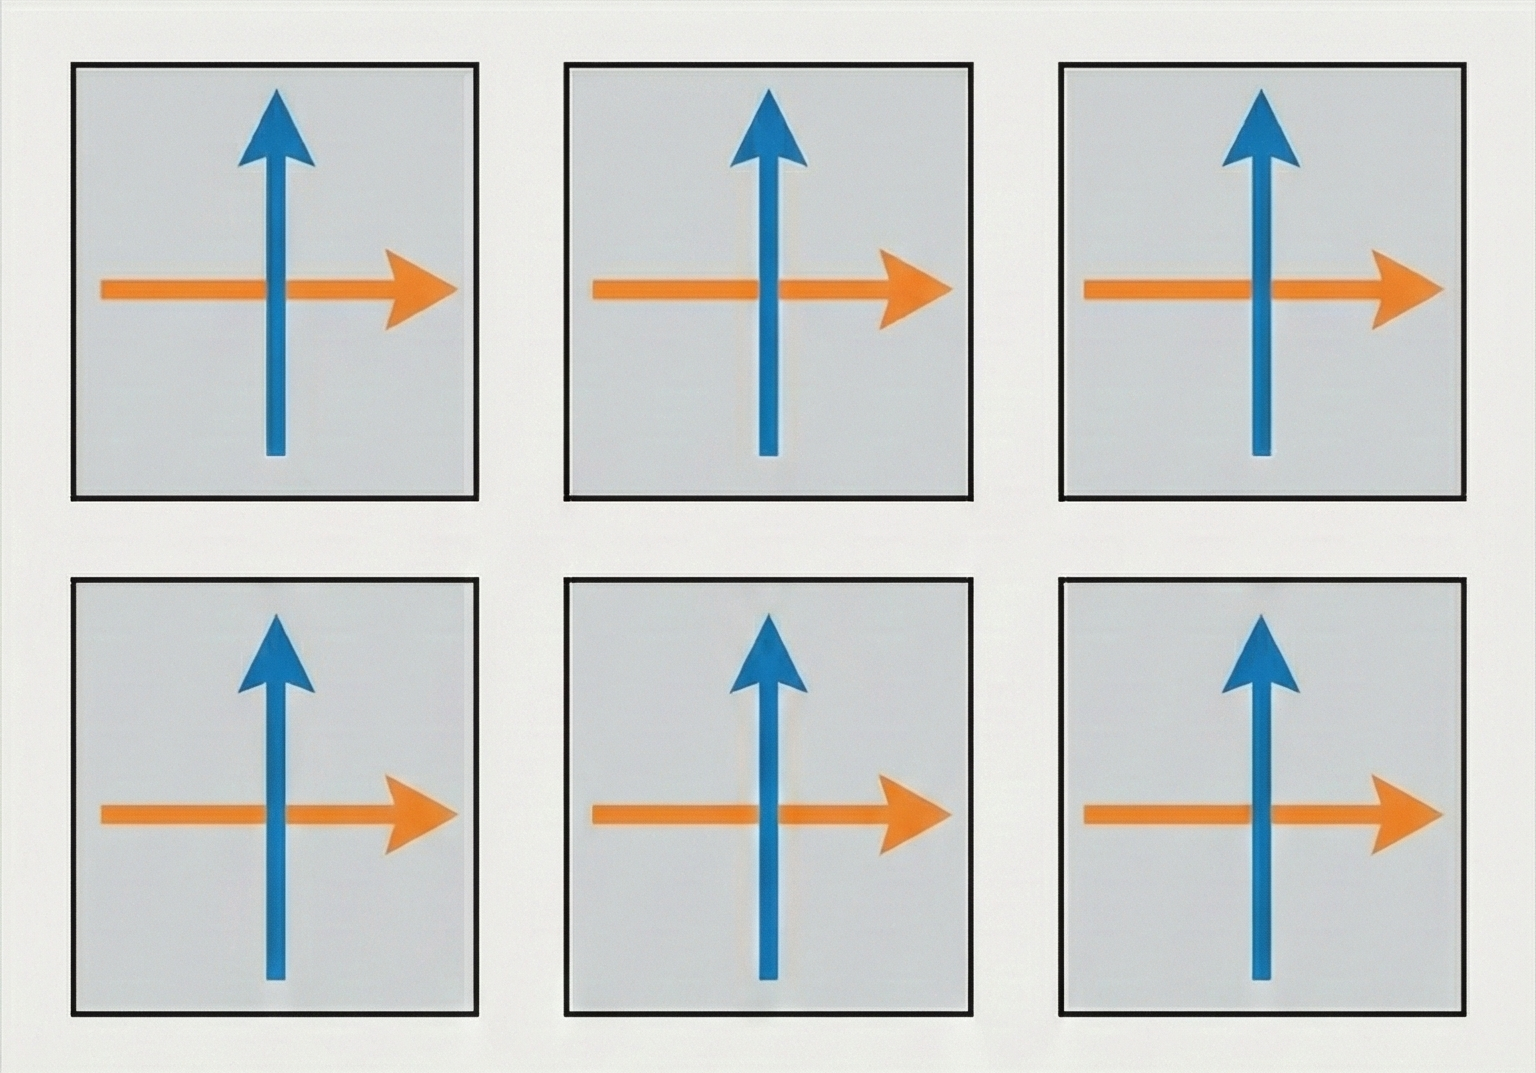
\includegraphics[height=.2\textheight]{images/dual_pol_elements.png}
        \caption{Dual-polarized elements}
        \label{fig:dual_pol_elements}
    \end{subfigure}
    ~
    \begin{subfigure}{0.45\textwidth}
        \centering
        
\includegraphics[height=.2\textheight]{images/interleaved_single_pol_elements.png}
        \caption{Interleaved single-polarized elements}
        \label{fig:interleaved_single_pol_elements}
    \end{subfigure}
    \\[2ex]
    \begin{subfigure}{\textwidth}
        \centering
        
\includegraphics[height=.23\textheight]{images/overlapping_single_pol_elements.png}
        \caption{Overlapping channels in an interleaved single-polarized element grid}
        \label{fig:overlapping_single_pol_elements}
    \end{subfigure}
    \caption{Comparison of physical element arrangements for polarimetric MIMO radar.}
\end{figure}


\subsection{Choice of radiating element and feeding platforms}

The survey of the literature, carried out in \cref{sec:frontend}, captures a vast and rapidly evolving design space for \qty{79}{GHz} automotive radar.
It is evident that emerging technologies, particularly \gls{gw} as an integration platform and \gls{med} as radiating elements, are maturing into robust solutions that address the traditional losses and bandwidth limitations of millimetre-wave circuitry.
These technologies represent the state of the art of electromagnetic design, offering superior isolation and polarization purity that are highly attractive for next-generation sensing.
However, the architectural choices for the specific research encompassed by this project are governed by a different set of optimization criteria.
The primary objective of this doctoral work is the extraction of dynamic, Doppler-resolved polarimetric signatures using a large-aperture \gls{mimo} radar.
In this context, the antenna array is not the primary subject of innovation but rather an enabler -- a critical functional block that must guarantee reliable data acquisition to validate the signal processing techniques of polarimetric decomposition and signature extraction.

Consequently, the focus is placed on the ability to rapidly prototype a complete, reliable polarimetric system with imaging capabilities, rather than employing experimental radiating elements that may introduce manufacturing uncertainties or integration delays.
To align with this objective, the following design decisions have been established:

\begin{itemize}
    \item \textbf{Adoption of planar technology.}
    To attain industrial support in terms of manufacturability and compatibility with standard calibration routines, the design is restricted to planar technologies (\gls{pcb}/\gls{ltcc}).
    While acknowledging the superior efficiency of air-filled waveguides, the mature fabrication processes of printed circuits ensure that the large-scale \gls{mimo} array can be produced with consistent tolerances, which is a prerequisite for accurate array manifold calibration.

    \item \textbf{Selection of radiating mechanism.}
    Within the planar domain, the design strategy envisions a multi-layer \gls{siw} stack-up as the high-performance contender.
    Specifically, slotted radiation serves as the main mechanism, potentially augmented with parasitic patches on the top layer to shape the individual beam pattern and improve impedance bandwidth, a technique supported by recent studies on hybrid \gls{siw}-patch topologies, such as works of~\textcite{puskely5GSIWBasedPhased2022,yangMillimeterWaveDualPolarizedDifferentially2020}.
    This approach strikes a balance between the isolation benefits of \gls{siw} and the low profile of printed elements.

    \item \textbf{Iterative development strategy.}
    To mitigate risk, particularly in the early phases of the project, the front-end design will leverage the established experience of dealing with uniform patch array cascades.
    This approach mirrors the proven architectures employed by industry leaders, such as Texas Instruments~\parencite{texasInstrumentsAwrxCascadedRadar2020} and Continental, for imaging automotive radar.
    By starting with a known baseline -- standard series-fed microstrip patches -- the research ensures a stable platform for initial data collection and algorithm development, allowing the focus to remain on the signal processing challenges of high-fidelity polarimetric measurements resolved in Doppler.
\end{itemize}

In summary, while the literature points toward \gls{gw} and \gls{med} as the future of automotive electromagnetics, this research purposefully selects established planar implementations to prioritize system-level reliability and the integrity of the polarimetric signal processing pipeline.


\section{Feasibility study and preliminary development}
\label{sec:feasibility-study}

To ground the proposed signal processing framework and topology synthesis in physical hardware, an initial experimental and simulation study was conducted.
This section details the development of a hybrid polarimetric scattering simulator and presents the electromagnetic design, parametric tuning, and full-wave verification of an aperture-coupled series-fed patch array baseline.


\subsection{Polarimetric scattering simulation model}
\label{sec:scattering-simulator}

To accurately model the full polarimetric response of electrically large target scenes%
    \footnote{Here, \enquote{electrically large target scenes} refers to isolated targets, such as a traffic sign located \qty{3}{\metre} from the antenna array, rather than complex automotive environments containing complex targets and environmental clutter. This representation remains valuable because even simple scenes are computationally intractable in full-wave solvers, necessitating the use of asymptotic solvers.}
and validate the decomposition algorithms prior to hardware testing, a dedicated simulation platform will be constructed.
The proposed technical pipeline employs a hybrid methodology, bridging full-wave electromagnetic data with an asymptotic ray-tracing solver within a unified software environment.
This approach ensures that array-level hardware physics are correctly accounted for while remaining computationally feasible for large-scale environments.
The pipeline is divided into three primary stages.

\paragraph{Antenna modelling via full-wave characterization.}
Rather than simulating the entire scene in a computationally expensive full-wave environment, a full-wave solver, namely the \gls{hfss} solver from the Ansys Electronics Desktop suite~\parencite{ansysAedt2025}, will be utilized exclusively to characterize the \gls{mimo} array.
This step is critical to capture exact electromagnetic properties that theoretical models cannot synthesize accurately, including mutual coupling, edge effects, and precise phase centre locations.
As a preliminary validation step, the simulator will replicate the \qty{28}{\giga\hertz} dual-polarized array specified by~\textcite{fandiantoroExperimentalStudyPolarimetric2025}.
This involves constructing an $8 \times 8$ array of dual-polarized elements (yielding a $16 \times 16$ port configuration) and extracting the complex embedded element patterns for all ports to serve as sources in the subsequent scattering simulation.

\paragraph{Scene scattering and propagation.}
Because targets such as \glspl{vru} are electrically massive at millimetre-wave frequencies, scene scattering will be evaluated using SBR+, an advanced \gls{sbr} solver integrated directly into the Ansys Electronics Desktop environment.
SBR+ traces electromagnetic rays from the transmitter to the target and back to the receiver via one-way coupling, accurately accounting for multiple surface reflections, edge diffractions, and creeping waves.
Operating within a single enterprise suite provides seamless integration: the complex 3D embedded radiation patterns calculated by \gls{hfss} are directly linked as far-field sources assigned to the transmitter and receiver coordinates in the SBR+ scene.
Initial validation will employ canonical shapes (e.g. spheres and dihedral corner reflectors) to verify the polarimetric scattering matrix extracted for each channel pair.

\paragraph{Integrated FMCW radar synthesis.}
A major architectural advantage of utilizing SBR+ within Ansys Electronics Desktop is its native support for dedicated \gls{fmcw} radar analysis setups.
Rather than manually synthesizing chirps, time delays, and phase shifts via external scripts, the SBR+ solver is configured directly with physical radar waveform parameters -- including sweep bandwidth, centre frequency, chirp duration, pulse repetition interval (\gls{pri}), number of chirps per frame, and frame period.
The solver automatically computes the multichannel \gls{fmcw} response and outputs raw Range-Doppler maps directly.
This eliminates tedious manual signal synthesis in Python, enabling post-processing scripts to focus directly on virtual array channel recombination, spatial imaging (e.g. back-projection), and target feature extraction.


\subsubsection{Staged simulation strategy}
\label{sec:staged-simulation-strategy}

To guarantee systematic progress and mitigate algorithmic risk, the evaluation of simulated and measured radar data will follow a staged processing pipeline, transitioning from fundamental power-based observables to advanced coherent decompositions.

\paragraph{Power-only reconstruction and phase calibration.}
Before deploying complex coherent target decompositions, initial simulations will establish a baseline using power-only polarimetric metrics (e.g. co-polar and cross-polar power ratios).
This initial stage focuses on resolving fundamental hardware-level challenges associated with single-polarized interleaved \gls{mimo} architectures, where orthogonal receive antennas are spatially displaced rather than sharing a common phase centre:
\begin{itemize}
    \item \textbf{Inter-element phase calibration:} Physical displacement between horizontal and vertical elements introduces an angle- and range-dependent path delay across the virtual array manifold. To enable accurate power ratio extraction across displaced channels, a dedicated calibration routine will be developed to compensate for these spatial phase shifts prior to channel combination.
    \item \textbf{Ensemble matrix averaging limits:} A critical theoretical challenge in calculating the polarimetric coherency matrix $\vec T = \langle \vec k_P \cdot \vec k_P^\dagger \rangle$ is defining the ensemble averaging operator $\langle \cdot \rangle$. In spaceborne \gls{sar}, averaging is performed spatially over large homogeneous terrain patches. In automotive radar, however, targets occupy only a few Range-Doppler resolution cells, restricting spatial multi-looking. Simultaneously, target motion and ego-vehicle dynamics cause rapid aspect angle variations that decorrelate phase within milliseconds, invalidating long temporal integration. The initial simulation phase will test localized Doppler-domain smoothing and spatial filtering techniques to form well-conditioned estimates under these constrained conditions.
\end{itemize}

\paragraph{Coherent polarimetric decomposition.}
Building upon the calibrated Range-Doppler data cubes and initial power-only baseline, the second phase will implement full coherent target decomposition techniques.
Custom post-processing scripts will apply \gls{mimo} spatial imaging algorithms (e.g. back-projection beamforming) to form full-aperture complex images.
Subsequently, multi-component incoherent decompositions -- such as the Yamaguchi four-component or Yamaguchi--Singh six-component methods -- will be applied to isolate physical scattering mechanisms (single-bounce, double-bounce, volume, and helix scattering) across dynamic \glspl{vru}.
This staged approach bridges initial power-only measurements with advanced polarimetric signal processing, explicitly validating how antenna non-idealities impact final target classification performance.


\subsection{Preliminary antenna design and development}

The transition from standard automotive radar to a fully polarimetric imaging system imposes stringent boundary conditions on the antenna element, primarily driven by a fundamental conflict between electromagnetic purity and industrial mass-producibility.
The core research question underpinning this design phase is the following: what constitutes a robust polarimetric antenna within the constraints of an automotive form factor?
While legacy systems prioritize forward gain and wide bandwidth, the extraction of reliable polarimetric signatures necessitates an \gls{xpd} exceeding \qty{20}{\decibel} across a wide \gls{fov}.
Consequently, the antenna cannot be treated merely as a passive component, but rather as a critical functional block that dictates the achievable dynamic range of the subsequent signal processing pipeline.

To align with the project's objective of validating signal processing algorithms on a reliable hardware platform, the proposed architecture purposefully builds upon the established planar topologies utilized in modern imaging automotive radars.
However, to overcome the inherent polarimetric limitations of standard series-fed patch arrays -- specifically, the degradation of \gls{xpd} caused by cross-polar radiation from feed networks -- this study adopts an aperture-coupled patch topology as the baseline design.
This baseline serves as the foundational stage in an iterative development strategy, which will eventually transition towards an \gls{siw} stack-up.


\subsubsection{Architectural rationale and element design}

The primary advantage of the aperture-coupled patch antenna architecture is its ability to physically and electromagnetically isolate the radiating patch from the feed network.
By separating the respective dielectric layers with a common ground plane, energy transfers magnetically through a ground-plane slot.
From an equivalent circuit perspective, the slot acts as a transformer representing the coupled impedance of the patch, connected in series with a parallel $LC$ resonant circuit that models the slot resonance and its associated fringing fields, all in series with the microstrip transmission line.
When plotted on a Smith chart, the input impedance locus of this composite structure typically forms a circle.
The primary objective of parametric tuning is to control the size and position of this circle, shifting it to pass directly through the centre of the Smith chart ($Z = 1$) to achieve a matched \qty{50}{\ohm} state.

A major benefit of this topology is the independent optimization of the feed and antenna substrates.
Ideally, the antenna substrate should be electrically thick ($h \ge \lambda_{0}/10$) with a low relative permittivity ($\epsilon_{\mathrm{r}} < 3$) to encourage outward radiation, widen the impedance bandwidth, and suppress surface-wave propagation, which is essential for maintaining channel isolation in \gls{mimo} arrays.
Conversely, the feed network requires an electrically thin substrate ($h < \lambda_{0}/50$) with a high permittivity ($\epsilon_{\mathrm{r}} > 5$) to confine the electromagnetic fields, maximize magnetic coupling through the aperture, and suppress spurious feed radiation.

Despite these guidelines, scaling the design to high-frequency bands reveals critical practical constraints that clash with theoretical ideals.
For instance, at lower microwave bands such as the X-band (e.g. \qty{9.7}{GHz}), a high-permittivity feed substrate like RO3006 ($\epsilon_{\mathrm{r}} = 6.5$) yields a practical width of \qty{0.38}{\milli\metre} for a \qty{50}{\ohm} microstrip line.
However, when scaling to the \qty{79}{GHz} automotive band, such a high permittivity forces the trace width to become microscopic, compounding conductor losses and exceeding standard \gls{pcb} fabrication tolerances.
Consequently, millimetre-wave arrays practically require a feed layer with a lower permittivity, typically between $\epsilon_{\mathrm{r}} = 3$ and $4$.

Furthermore, high-frequency scaling introduces severe surface-wave vulnerabilities.
At \qty{9.7}{GHz} on a \qty{787}{\micro\metre} RO3006 substrate, the substrate electrical thickness ($\approx 0.025\lambda_{0}$) naturally excites the dominant $\text{TM}_{0}$ surface-wave mode.
While this can cause scan blindness in large \gls{mimo} arrays (e.g. $8 \times 4$), it remains manageable.
At \qty{79}{GHz}, the $h/\lambda_{0}$ ratio increases substantially.
Without drastic substrate thinning, higher-order modes (such as $\text{TE}_{1}$) cut on, leading to severe power dissipation, mutual coupling, and spatial decorrelation that degrades the virtual aperture.
Transitioning to a \gls{siw} cavity-backed topology provides a metallic wall boundary that completely suppresses lateral surface waves, representing the ultimate solution for preserving virtual array integrity.
As frequency increases or as the substrate becomes electrically thicker, higher-order modes cut on.
The cutoff frequency for the $\text{TE}_{n}$ modes is given by
\begin{equation}
    f_{c,\text{TE}_n} = \frac{(2n-1)c}{4h\sqrt{\epsilon_{\mathrm{r}} - 1}},
\end{equation}
where $c$ is the speed of light in vacuum, $h$ is the substrate thickness, and $\epsilon_{\mathrm{r}}$ is the relative permittivity.
At \qty{79}{GHz}, the wavelength $\lambda_{0}$ is roughly \qty{3.8}{\milli\metre}; if the substrate thickness $h$ is not kept thin, the physical thickness easily exceeds the cutoff threshold for $\text{TE}_{1}$, allowing it to propagate and affect the array's mutual coupling.

\paragraph{Parametric tuning.}
Tuning the aperture-coupled antenna within a full-wave electromagnetic solver requires mapping the physical dimensions of the structure to its electrical response.
The patch length acts as the primary control for the operating frequency, to which it is inversely proportional; even a \qty{0.1}{\milli\metre} variation at X-band drastically shifts the resonance, demanding high tuning precision.
The patch width primarily controls the resonant resistance, with a wider patch leading to a lower input resistance.
The slot length serves as the primary control for the coupling coefficient, and increasing it expands the diameter of the impedance locus on the Smith chart.
However, the slot must remain strictly sub-resonant (ideally $\approx \lambda_{\mathrm{g}}/10$) to suppress excessive back-radiation.
If a half-wavelength slot ($\lambda_{\mathrm{g}}/2$) is required to achieve matching, it typically indicates that the feed substrate is too thick or its permittivity too low.
The slot width has a minor influence on coupling, and a standard aspect ratio of approximately $10:1$ is maintained, though modifying the slot to an hourglass or bow-tie shape can increase magnetic polarizability without expanding the physical footprint.
Finally, the feed stub length past the slot is used to tune out excess slot reactance.
Although classical one-dimensional theory dictates a length slightly less than $\lambda_{\mathrm{g}}/4$, localized dielectric loading and fringing capacitance can reduce the actual physical length to merely \qtyrange{35}{40}{\percent} of the theoretical quarter-wavelength.
Shortening the stub rotates the impedance locus downwards in the capacitive direction on the Smith chart.

In practice, several tuning strategies can be employed.
Rather than forcing a high-Q match exactly at $Z = 1$, the coupling can be intentionally increased by lengthening the slot.
This causes the impedance loop to intersect the $R=1$ circle at two symmetric points, broadening the operating bandwidth.
Furthermore, changing the slot length alters its reactance, which must be counteracted by re-tuning the feed stub length, while slot-induced resonance pulling requires slight patch length adjustments to re-centre the operating frequency.

\subsubsection{Series-feed synthesis}

Transitioning from a single aperture-coupled patch to a series-fed array transforms the structure from a localized load into a cascaded microwave network.
In a series configuration, intermediate elements do not possess individual tuning stubs; the feedline simply traverses the slot and continues.
The termination after the final element dictates the array's behaviour.
\begin{itemize}
    \item \emph{Standing-wave arrays} terminate the feedline with an open-ended tuning stub after the final element to establish a standing wave, which is highly radiation-efficient but limits the impedance bandwidth to typically \qtyrange{1}{2}{\percent} because frequency shifts cause the standing-wave nodes to drift away from the slot positions.
    \item \emph{Travelling-wave arrays} terminate the feedline with a matched \qty{50}{\ohm} load to absorb residual power, preventing standing waves and securing a wider impedance bandwidth, though the main beam inherently squints with frequency, which is detrimental to \gls{fmcw} radar angular resolution.
\end{itemize}
In theory, this beam squint can be eliminated in centre-fed travelling-wave configurations due to symmetric cancellations.
Crucially, confining the feed network behind a solid ground plane in an aperture-coupled series topology suppresses feed network radiation, yielding the high \gls{xpd} required for polarimetric applications.

However, series-fed travelling-wave arrays terminated in a matched load present a fundamental design paradox when configured to radiate broadside.
In-phase broadside radiation requires the electrical length of the interconnects between elements at the feeding layer to equal an integer multiple of the guided wavelength ($L = n\lambda_{\mathrm{g}}$).
Under this condition, localized reflections from each slot travel back to the input, and because the round-trip distance is $2n\lambda_{\mathrm{g}}$, these reflections add constructively, generating a massive input reflection that destroys the travelling-wave condition.
Conversely, introducing a phase shift to squint the beam off-broadside introduces a phase mismatch that causes reflections to interfere destructively at the input, yielding excellent return loss but pointing the main beam off-broadside.
To resolve this conflict, two architectural paths are available: maintaining the travelling-wave topology for bandwidth while applying a progressive phase shift to squint the beam slightly off-broadside in elevation, which can be compensated for mechanically, or switching to a standing-wave topology by removing the progressive phase shift and integrating a dedicated input matching network to match the real input impedance to the system impedance.

\paragraph{Amplitude tapering.}
In series-fed travelling-wave arrays, the power propagates along the feedline and is sequentially leaked or extracted by each successive slot element.
As the electromagnetic wave travels down the array, the power remaining in the feedline decreases.
Consequently, each subsequent element has less available power to extract than its predecessor.
This behaviour is fundamentally different from resonant standing-wave arrays, where a stationary wave pattern is established, and element excitations are dictated by the global standing-wave profile rather than sequential loss.
To achieve a specific amplitude taper, such as a Taylor or Chebyshev distribution, the coupling strength of the elements must be graded, requiring the initial elements to be weakly coupled and the terminal elements to be strongly coupled.
This gradient is quantified by the \gls{rapr}, defined as the ratio of the power radiated by an element to the power available to it.
The array synthesis involves calculating the desired \gls{rapr} profile to achieve the target \gls{sll} and mapping it to physical dimensions.
To cover the required dynamic range of \gls{rapr}, which typically ranges from $< \qty{1}{\percent}$ near the feed point to $> \qty{70}{\percent}$ at the terminal end, the array must employ different element types to manage both high and low coupling states without introducing reflections, as demonstrated for travelling-wave array synthesis with three element types to cover the wide \gls{rapr} range required for automotive beams~\parencite{kangDesignTravelingWaveSeriesFed2020}.

Sweeping standard rectangular slot dimensions reveals coupling limits.
While low-coupling elements can extract down to \qty{0.45}{\percent} of the power, the peak coupling of standard rectangular slots terminates at \qtyrange{20}{30}{\percent}.
For small arrays, this coupling limit is highly problematic.
In a series-fed travelling-wave array with a small element count (e.g. $N = 7$), each element must extract a large fraction of the remaining power to achieve high radiation efficiency.
This constraint is exacerbated by amplitude tapering, as the central elements are responsible for radiating the majority of the power.
If the maximum coupling is restricted to $\approx \qty{25}{\percent}$, the central elements cannot extract enough energy.
Consequently, the target taper can only be satisfied by allowing a substantial fraction of the input power (approximately \qtyrange{40}{50}{\percent}) to propagate past the slots and dissipate as heat in the terminal load, dropping the overall radiation efficiency to approximately \qty{50}{\percent}.
Conversely, in larger arrays ($N > 20$) or standing-wave resonant arrays, a maximum coupling of \qty{24.4}{\percent} is entirely sufficient because the power is distributed across more elements or recycled via standing waves.
For small travelling-wave arrays, however, slot modifications are necessary to increase the coupling coefficient.

\paragraph{Coupling characterization.}
To map the physical dimensions of each patch and slot to the required coupling coefficients, single elements are characterized in a two-port unit-cell environment.
Assuming a lossless network, the \gls{acc}, denoted $|C|^2$, is extracted from the scattering parameters:
\begin{equation}
    |C|^2 = 1 - |S_{11}|^2 - |S_{21}|^2.
\end{equation}
Reference planes in the full-wave solver must be de-embedded to the centre of the slot to remove phase rotation and feedline loss.
Additionally, the slot must remain sub-resonant, and second-pass optimization is required to account for mutual coupling loading effects between adjacent patches.

\paragraph{Phase matching.}
To generate a standard automotive fan beam pointing broadside without grating lobes, the physical and electrical spacing must be decoupled.
The element spacing $d$ must be kept at approximately $0.5\lambda_{0}$, and strictly below $\lambda_{0}$, to prevent grating lobes, while the elements must be fed in phase, requiring a $2\pi+\Phi_{\mathrm{prog}}$ electrical delay, where $\Phi_{\mathrm{prog}}$ is the intended progressive phase.
Because the guided wavelength is shorter than the free-space wavelength in the substrate, meanders or U-bends are routed between the slots to physically lengthen the line.
In travelling-wave arrays, tuning elements to different coupling levels shifts their transmission and radiation phases, and realizing an accurate beam pattern requires tracking the radiation phase, $\angle E_{\mathrm{rad}}$, of each element.
To maintain the progressive phase, $\Phi_{\mathrm{prog}}$, the electrical length, $\Delta\Phi_{\mathrm{feed}}$, of the feedline segment between elements $i$ and $i+1$ is synthesized as
\begin{equation}
    \Delta\Phi_{\mathrm{feed}} = \angle S_{21,i} + \angle E_{\mathrm{rad},i+1} - \angle E_{\mathrm{rad},i} - \Phi_{\mathrm{prog}}.
\end{equation}

\paragraph{Array scaling limits.}
When scaling the array, two parameters dictate performance bounds.
First, increasing the element count $N$ smooths the amplitude taper and reduces the required peak coupling, enhancing radiation efficiency, but as the feedline length increases, cumulative dielectric and conductor insertion losses begin to outpace the directivity gain.
For X-band arrays on RO3006, realized gain typically saturates between $12$ and $16$ elements.
Second, setting the spacing $d \approx \lambda_{0}$ increases directivity but is detrimental, as any frequency-induced squint will immediately steer a grating lobe into the visible region, and the longer interconnecting lines increase the phase slope, worsening frequency dispersion.
Spacing is therefore restricted to the $0.5\lambda_{0}$ to $0.7\lambda_{0}$ range.

\subsubsection{High-coupling elements and series impedance matching}

Achieving the high coupling levels required for tapered arrays (where \gls{rapr} exceeds \qty{70}{\percent}) introduces complex series slot impedances ($Z_{\mathrm{slot}} = R_{\mathrm{slot}} + \ii X_{\mathrm{slot}}$) that generate reflections and disrupt the travelling-wave distribution.

To achieve high coupling without reflections, a two-part feedline modification is implemented.
First, to maximize magnetic coupling, a modified-hourglass shape of coupling aperture is used to reach high values of aperture coupling~\parencite{priyalathaCompactModifiedHourglassshaped2023}, and the microstrip line is narrowed (e.g. to \qty{0.1}{\milli\metre}) strictly over the slot, increasing current density and magnetic flux.
Second, an integrated impedance transformer is placed immediately upstream of the slot.
A series slot impedance $Z_{\mathrm{slot}}$ in series with the continuing line creates a total load $Z_{L} = Z_{0} + Z_{\mathrm{slot}}$.
For an element extracting \qty{70}{\percent} of the power, this series impedance is approximately $2.33 Z_{0}$ ($\approx \qty{116}{\ohm}$), resulting in a total load of $\approx \qty{166}{\ohm}$.
To match this to the incoming line, the integrated microstrip transformer is placed immediately upstream, while the line immediately downstream of the slot returns to the nominal $Z_{0}$ width to act as the continuation load.

Assuming the composite coupler acts as a series impedance, the slot impedance is extracted from two-port S-parameters as%
\footnote{For $Z_{0}$, we utilize the simulated line impedance ($Z_{\mathrm{line}}$) rather than an ideal \qty{50}{\ohm} to avoid systematic phase errors.}
\begin{equation}
    Z_{\mathrm{slot}} = 2 Z_{0} \frac{S_{11}}{1 - S_{11}}.
\end{equation}
By equating the input impedance of the preceding transformer (of impedance $Z_1$ and electrical length $\theta$) to the line impedance $Z_0$, we obtain
\begin{equation}
    Z_{0} = Z_{1} \frac{(Z_{0} + R_{\mathrm{slot}} + \ii X_{\mathrm{slot}}) + \ii Z_{1} \tan\theta}{Z_{1} + \ii (Z_{0} + R_{\mathrm{slot}} + \ii X_{\mathrm{slot}}) \tan\theta}.
\end{equation}
Solving the real and imaginary parts yields the required transformer electrical length and impedance:
\begin{align}
    Z_{1} &= \sqrt{Z_{0}^2 + \frac{Z_{0}}{R_{\mathrm{slot}}} \( R_{\mathrm{slot}}^2 + X_{\mathrm{slot}}^2 \) },
&
    \tan\theta &= -\frac{Z_{1} R_{\mathrm{slot}}}{Z_{0} X_{\mathrm{slot}}}.
\end{align}
Unlike standard quarter-wave equations, this derivation accounts for the additive series load $Z_{L} = Z_{0} + Z_{\mathrm{slot}}$, collapsing back to the geometric mean if the line were terminated ($Z_{0} \rightarrow 0$).
To automate array synthesis, the search space is divided into three families: a high-coupling regime (up to \qty{-2}{dB} \gls{acc}) employing the thinned line and quarter-wave transformer; a vanilla hourglass regime (up to \qty{-4}{dB} \gls{acc}) where the transformer and thinned section are disabled, and coupling is tuned purely by the hourglass flare width; and a simple slot regime (\qty{-6}{dB} \gls{acc} and below) employing standard rectangular slots, tuned via slot width.
In all cases, the slot length is swept with fine resolution to ensure the optimizer identifies the frequency where $\Im(Z_{\mathrm{slot}}) \approx 0$.

\subsubsection{Simulation results and architectural transition}

An $N = 8$ series-fed travelling-wave array was synthesized at \qty{9.7}{GHz} using modified-hourglass slots, localized trace thinning, and integrated series transformers, and characterized using full-wave electromagnetic simulation sweeps of the progressive phase shift.
The return loss and bandwidth results of the phase sweep are summarized in \cref{tab:return_loss_bandwidth}.
At the designed progressive phase of $\ang{-15.0}$, the array achieves an input match of \qty{-12.40}{dB} at \qty{9.7}{GHz}, but with a narrow operating bandwidth of only \qty{0.82}{\percent} (\qty{80}{MHz}).
For all other phase angles, the match collapses ($S_{11} > \qty{-10}{dB}$).
This high sensitivity is attributed to the cascaded quarter-wave matching sections: slight deviations from the design frequency rotate the impedance locus, causing reflections to add constructively at the input.

\begin{table}[ht]
    \centering
    \caption{Return loss and bandwidth collapse of the aperture-coupled patch array under progressive phase variation at \qty{9.7}{GHz}}
    \label{tab:return_loss_bandwidth}
    \small
    \begin{tabular}{ccccc}
        \toprule
        $\Phi_{\mathrm{prog}}$ (\unit{\degree}) & $S_{11}$ (dB) & BW (\%) \\
        \midrule
        $-15.0$ & $-12.40$ & $0.82$ \\
        $-10.0$ & $-7.77$  & $0.00$ \\
        $-5.0$  & $-5.51$  & $0.00$ \\
        $0.0$   & $-4.36$  & $0.00$ \\
        $5.0$   & $-3.80$  & $0.00$ \\
        $10.0$  & $-3.93$  & $0.00$ \\
        $15.0$  & $-3.01$  & $0.00$ \\
        \bottomrule
    \end{tabular}
\end{table}

The radiation pattern metrics are detailed in \cref{tab:radiation_performance}.
At $\ang{-15.0}$, the phase compensation successfully steers the main beam to broadside (\ang{0.0} squint) with a peak gain of \qty{12.77}{dBi} and an azimuth \gls{sll} of \qty{-12.65}{dB}.
The fact that broadside steering coincides with the best input match indicates that the feed network phase compensation aligns both radiation phases and input reflection cancellation.
Polarization purity remains high, exceeding \qty{30}{dB} across the azimuth scan ($\varphi \in [\ang{-90}, \ang{90}]$, $\theta \in [\ang{-15}, \ang{15}]$), confirming the shielding effectiveness of the ground plane.

\begin{table}[ht]
    \centering
    \caption{Radiation performance of the aperture-coupled patch array under progressive phase variation at \qty{9.7}{GHz}}
    \label{tab:radiation_performance}
    \small
    \begin{tabular}{ccccc}
        \toprule
        $\Phi_{\mathrm{prog}}$ (\unit{\degree}) & Gain (dBi) & Squint (\unit{\degree}) & \gls{sll} (dB) \\
        \midrule
        $-15.0$ & $12.77$ & $0.0$  & $-12.65$ \\
        $-10.0$ & $12.17$ & $0.0$  & $-12.05$ \\
        $-5.0$  & $11.39$ & $-5.0$ & $-11.75$ \\
        $0.0$   & $10.95$ & $-5.0$ & $-11.36$ \\
        $5.0$   & $10.63$ & $-5.0$ & $-10.98$ \\
        $10.0$  & $10.76$ & $-5.0$ & $-10.20$ \\
        $15.0$  & $10.16$ & $-5.0$ & $-10.14$ \\
        \bottomrule
    \end{tabular}
\end{table}

The bandwidth collapse (\qty{0.82}{\percent}) indicates that while the matching transformers achieve high coupling, they compromise the bandwidth of the travelling-wave array.
Two solutions are proposed to resolve this limitation.
First, the design can transition to a centre-fed series-corporate hybrid topology.
Splitting the input port symmetrically at the array centre (using a corporate T-junction on an underlying layer) to feed two identical series branches propagating outwards aligns the peak power requirement with the physical feed location.
This reduces and flattens the required coupling coefficients, removing the need for high-ratio transformers or thinned feedlines, and preserving the array's wide bandwidth.
Additionally, frequency-induced squint on the symmetric branches is equal and opposite, cancelling the overall beam squint.
Second, transverse shunt-stub matching networks can replace the longitudinal transformers.
Although stubs can offer a broader impedance match, they add layout complexity and increase the risk of coupling with adjacent patch cavities.
Finally, to improve the \gls{rapr} capabilities of a single terminal element, the performance of the terminal virtual load element should be investigated, as terminal element improvements will be highly visible in the side-fed architecture, paving the way for a high-efficiency centre-fed design.
